\documentclass[11pt,pdftex,twoside,letterpaper]{exam}
\usepackage{amsmath,amssymb, amsthm}
%\usepackage{ccfonts,eulervm}
%\usepackage[T1]{fontenc}
\usepackage{graphicx}
\usepackage{xcolor}
\usepackage{booktabs}
\usepackage{caption}
\usepackage{setspace}
\usepackage[compact]{titlesec}
\usepackage{enumitem}
\usepackage{mdframed}
\usepackage[colorlinks=true,linkcolor=blue,citecolor=black,urlcolor=blue,bookmarks=false,pdfstartview={FitV}]{hyperref}
\usepackage{placeins}
\usepackage{cancel}
\usepackage{array}
\usepackage{float}
\usepackage{multirow}
\usepackage[many]{tcolorbox}
\usepackage{subcaption}
\usepackage{tikz}

\newtcolorbox{mybox}[1]{%
    tikznode boxed title,
    enhanced,
    arc=0mm,
    interior style={white},
    attach boxed title to top center= {yshift=-\tcboxedtitleheight/2},
    fonttitle=\bfseries,
    colbacktitle=white,coltitle=black,
    boxed title style={size=normal,colframe=white,boxrule=0pt},
    title={#1}}


%%%%%%%%%%%%%%%%%%%%%%%%%%%%%%%%%%%%%%%%%%%%%%%%%%%%%%%%%%%%%%%%%%%%%%%%%%%%%
\renewcommand{\CancelColor}{\color{red}}

\DeclareRobustCommand{\bbone}{\text{\usefont{U}{bbold}{m}{n}1}}
\DeclareMathOperator{\EX}{\mathbb{E}}% expected value
\DeclareMathOperator{\std}{\mathrm{std}}
\DeclareMathOperator{\cov}{\mathrm{cov}}
\DeclareMathOperator{\corr}{\mathrm{corr}}
\DeclareMathOperator{\var}{\mathrm{var}}

%%%%%%%%%%%%%%%%%%%%%%%%%%%lists%%%%%%%%%%%%%%%%%%%%%%%%%%%%%%%%%%%%%%%%%%%%%%
%\setlist{nosep}        %no space anywhere --- too extreme for me
\setlist[description, 1]{itemsep=1ex}
\setlist[description]{topsep=0ex}
\setlist[itemize]{topsep=0ex}
\setlist[enumerate]{topsep=0ex, itemsep=0.0ex}
%%%%%%%%%%%%%%%%%%%%%%Margins%%%%%%%%%%%%%%%%%%%%%%%%%%%%%%%%%%%%%%%%%%%%%%%
\usepackage[top=1.25in, bottom=1.0in, left=1.0in, right=1.0in]{geometry}
\setlength{\parindent}{0in}
\setlength{\parskip}{\bigskipamount}
\raggedbottom

%titlesec definitions
\titlespacing*\section{0pt}{1pt plus 0pt minus 0pt}{0pt plus 0pt minus 0pt}
\titlespacing*\subsection{0pt}{1pt plus 0pt minus 0pt}{0pt plus 0pt minus 0pt}
\titlespacing*\subsubsection{0pt}{0pt plus 2pt minus 2pt}{0pt plus 2pt minus 2pt}

%%%%%%%%%%%%%%%%%%%%%%Headers and Footers%%%%%%%%%%%%%%%%%%%%%%%%%%%%%%%%%%
\pagestyle{headandfoot}
\runningheadrule
%\firstpageheadrule
% use "/" rather than the windows "\" in paths.
\firstpageheader{}{}{}%{\textbf{International \\ Macroeconomics}\vspace{0.0cm}}
%{\includegraphics[width=0.35\textwidth]{C://Users//kjr42//Dropbox//Tools//PS_HOR_RGB_Black.png}}
\runningheader{\textbf{Two-country models}}{}{}
\runningfooter{}{}{pg: \thepage}


%%%%%%%%%%%%%%%%%%%%%%%%%%%%%%%%%%%%%%%%%%%%%%%%%%%%%%%%%%%%%%%%%%%%%%%%%%%%%%%%%%%%%%%%%%%%%%%%%%%%%%%%%%%%%%%%%%%%%%%%%%%%%%%%%%%%
\begin{document}

\centerline{\Large Two-country open economy models}%
\smallskip
\centerline{This version: \today}

\section{Endowment economies}
The model consists of two equally-sized countries, home and foreign, and two non-storable and freely tradable goods, $x$ and $y$. [We will introduce trade frictions and production shortly.] The goods come from two trees: the $x$ tree is in the home country and the $y$ tree is in the foreign country. Uncertainty over the output of the trees follows the usual notation, a state is $s_t\in S$ and $s^t=(s_0,s_1,\ldots s_t)$ is a history. $\pi(s^t)$ is probability (conditional on $s_0$) of being in  history $s^t$.

The resource constraints are
\begin{eqnarray}
% \nonumber % Remove numbering (before each equation)
  X(s^t) &=& x(s^t)+x^*(s^t) \label{eq:bcx}\\
  Y(s^t) &=& y(s^t)+y^*(s^t) \label{eq:bcy}
\end{eqnarray}
where a $^*$ denotes a foreign-country variable. Preferences are
\begin{eqnarray}
% \nonumber % Remove numbering (before each equation)
  V_0\left(x\left(s^t\right), y\left(s^t\right)\right) &=&  \sum_{t=0}^\infty \sum_{s^t} \beta^t \pi(s^t)u\left( x\left(s^t\right), y\left(s^t\right) \right)
\end{eqnarray}
for the home country with analogous specification for the foreign country. The discount factor, strictly concave utility function, and probabilities are common across countries. We assume that the utility functions imply risk aversion so agents would like to use security markets to pool risk with each other.

\subsection{Social planner's problem}
A benevolent planner solves
\begin{eqnarray}
% \nonumber % Remove numbering (before each equation)
  \max_{x, y, x^*, y^*} &=& \lambda V_0\left(x\left(s^t\right), y\left(s^t\right)\right) + (1-\lambda)V_0\left(x^*\left(s^t\right), y^*\left(s^t\right)\right)
\end{eqnarray}
subject to \eqref{eq:bcx} and \eqref{eq:bcy}. The $\lambda$ terms are the Pareto weights assigned to each country. Notice that this maximand can be written
\begin{eqnarray}
% \nonumber % Remove numbering (before each equation)
  \max_{x, y, x^*, y^*} &=&  \sum_{t=0}^\infty \sum_{s^t} \beta^t \pi(s^t) \left \{ \lambda u(x(s^t),y(s^t)) + (1-\lambda) u(x^*(s^t),y^*(s^t))   \right \}
\end{eqnarray}
which means that this is a state-by-state decision problem. This requires time seperability in preferences. So solve
\begin{eqnarray}
% \nonumber % Remove numbering (before each equation)
  \max_{x, y, x^*, y^*} &=&  \lambda u\left(x(s^t),y(s^t) \right) + (1-\lambda) u\left(X(s^t)-x(s^t),Y(s^t)-y(s^t)\right)
\end{eqnarray}
for all $s^t$. The first-order conditions are
\begin{eqnarray}
% \nonumber % Remove numbering (before each equation)
  \lambda u_x(s^t) &=& (1-\lambda)u_x^*(s^t)\\
  \lambda u_y(s^t) &=& (1-\lambda)u_y^*(s^t)
\end{eqnarray}
which implies that
\begin{eqnarray}
% \nonumber % Remove numbering (before each equation)
  \frac{1-\lambda}{\lambda} &=& \frac{u_x(s^t)}{u_x^*(s^t)}=\frac{u_y(s^t)}{u_y^*(s^t)} \label{eq:planners-cond}
\end{eqnarray}
Since preferences do not connect future or past consumption with present utility, the planner in each history takes the total output of a good and splits it between the agents to equalize marginal utility with their relative Pareto weight. If $\lambda=0.5$, consumption is equalized across countries.

By varying $\lambda$ between zero and one, we trace out all of the Pareto optimal allocations.

Planner's problems are nice because they are easy to solve. This allocation requires solving, for each $s^t$, four equations in four unknowns.  We are often interested in market equilibria. Let's turn to some decentralizations of this allocation.
\subsection{Arrow-Debreu equilibrium}
 At time zero, agents commit to a set of trades that are contingent on the history that occurs. The home country solves
 \begin{eqnarray}
% \nonumber % Remove numbering (before each equation)
  V_0\left(x\left(s^t\right), y\left(s^t\right)\right) &=&  \sum_{t=0}^\infty \sum_{s^t} \beta^t \pi(s^t)u\left( x\left(s^t\right), y\left(s^t\right) \right)
\end{eqnarray}
\begin{eqnarray}
% \nonumber % Remove numbering (before each equation)
  \textrm{s.t.} \;\; \sum_{t=0}^\infty \sum_{s^t} m(s^t)\left[ x(s^t)+p(s^t)y(s^t)  \right]&=& \sum_{t=0}^\infty \sum_{s^t} m(s^t) X(s^t)
\end{eqnarray}
The foreign country maximizes utility subject to
\begin{eqnarray}
% \nonumber % Remove numbering (before each equation)
  \sum_{t=0}^\infty \sum_{s^t} m(s^t)\left[ x^*(s^t)+p(s^t)y^*(s^t)  \right]&=& \sum_{t=0}^\infty \sum_{s^t} m(s^t) p(s^t)Y(s^t)
\end{eqnarray}
where the relative price of good $y$ to $x$ is $p$. Note that this is also the home country's terms of trade and the inverse of the foreign country's terms of trade. [Todo: This is a change in definition from earlier notes. Make these consistent.] The price of good $x$ is $m$.

Assign $\gamma$ and $\gamma^*$ as multipliers to the budget constraints. The first-order conditions are
\begin{eqnarray}
% \nonumber % Remove numbering (before each equation)
  \beta^t\pi(s^t)u_x(s^t) &=& \gamma m(s^t) \\
  \beta^t\pi(s^t)u_y(s^t) &=& \gamma m(s^t) p(s^t)\\
  \beta^t\pi(s^t)u_x^*(s^t) &=& \gamma^* m(s^t) \\
  \beta^t\pi(s^t)u_y^*(s^t) &=& \gamma^* m(s^t) p(s^t)
\end{eqnarray}
These imply that
\begin{eqnarray}
% \nonumber % Remove numbering (before each equation)
  \frac{\gamma}{\gamma^*} =\frac{u_x(s^t)}{u_x^*(s^t)} = \frac{u_y(s^t)}{u_y^*(s^t)}
\end{eqnarray}
and we have state-by-state equalization of marginal utility. Note that because the $\gamma$'s are constant, marginal utility is equated over time. This is perfect risk sharing. Only aggregate risk matters here.
\subsection{Sequence of markets}
Assume that there are a set of Arrow securities (a set of one-period bonds, each one paying off only if one state occurs in the next period). We assume that each country is endowed with an initial asset, $a(s_0)$.

The home country maximizes utility subject to, for every $s^t$,
\begin{eqnarray}
% \nonumber % Remove numbering (before each equation)
  x(s^t) + p(s^t)y(s^t) +\sum_{s^{t+1}|s^t}q(s^t,s^{t+1})a(s^{t+1})&=& a(s^t)+X(s^t).
\end{eqnarray}
Arrow security $a(s^t,s^{t+1})$ pays one unit of $x$ if state $s^{t+1}$ follows state $s^t$ and zero otherwise. It's price is $q(s^t,s^{t+1})$. The foreign country has the budget constraint
\begin{eqnarray}
% \nonumber % Remove numbering (before each equation)
  x^*(s^t) + p(s^t)y^*(s^t) +\sum_{s^{t+1}|s^t}q(s^t,s^{t+1})a^*(s^{t+1})&=& a^*(s^t)+Y(s^t).
\end{eqnarray}
An equilibrium is $\{q, p, a, a^*, x, x^*, y, y^*\}$ such that, given $\{q,p\}$ allocations $\{a, a^*, x, x^*, y, y^*\}$ solve the home and foreign country maximization problems, good markets clear, and assets are in zero net supply,
\begin{eqnarray}
% \nonumber % Remove numbering (before each equation)
  a(s^t)+ a^*(s^t)=0.
\end{eqnarray}
The transversality condition for the home country is
\begin{eqnarray}
% \nonumber % Remove numbering (before each equation)
  \lim_{T\rightarrow\infty}\sum_{s^{T+1}}\left( \prod_{t=0}^T q(s^t,s^\prime)\right)a(s^{T+1})=0
\end{eqnarray}
with an analogous expression for $a^*(s^{T+1})$. [Todo: sort out the notation for $q$.]

The first-order conditions from this problem are
\begin{eqnarray}
% \nonumber % Remove numbering (before each equation)
  \beta^t\pi(s^t)u_x(s^t) &=& \gamma(s^t) \\
  \beta^t\pi(s^t)u_y(s^t) &=& \gamma(s^t) p(s^t)\\
  \beta^t\pi(s^t)u_x^*(s^t) &=& \gamma^*(s^t) \\
  \beta^t\pi(s^t)u_y^*(s^t) &=& \gamma^*(s^t)  p(s^t)
\end{eqnarray}
At this point we have
\begin{eqnarray}
% \nonumber % Remove numbering (before each equation)
  \frac{u_x(s^t)}{u_x^*(s^t)} = \frac{u_y(s^t)}{u_y^*(s^t)} = \frac{\gamma(s^t)}{\gamma^*(s^t)}
\end{eqnarray}
but the $\gamma$ terms still have $s^t$ in them. They could be time-varying.

The first-order condition for bonds implies that the ratio of the multipliers is constant over time
\begin{eqnarray}
% \nonumber % Remove numbering (before each equation)
  \gamma(s^t)q(s^t,s^{t+1}) &=& \gamma(s^{t+1})\\
  \gamma^*(s^t)q(s^t,s^{t+1}) &=& \gamma^*(s^{t+1})
\end{eqnarray}
so the ratio of marginal utilities is constant over time, and again we have perfect risk sharing.
\begin{eqnarray}
% \nonumber % Remove numbering (before each equation)
  \frac{u_x(s^t)}{u_x^*(s^t)} &=& \frac{u_x(s^{t+1})}{u_x^*(s^{t+1})}\\
  \frac{u_y(s^t)}{u_y^*(s^t)} &=& \frac{u_y(s^{t+1})}{u_y^*(s^{t+1})}
\end{eqnarray}
Note that the consumption levels, however, depend on the initial wealth levels of each country, $a(s_0)$ and $a^*(s_0)$.

\subsection{Planner's problems and equilibria}
With complete markets (either Arrow-Debreu or sequential) we can achieve the perfect risk sharing that the planner would choose. This is an expression of the first welfare theorem: the competitive equilibrium is optimal.

The second welfare theorem also holds, and suggests a way to compute an equilibrium that supports the planner's allocation. This is known as the Negishi-Mantel algorithm. The idea is that the social planner's problem does not respect the budget constraint. Finding a competitive equilibrium given a planner's allocation requires finding a transfer of wealth from one country to the other so that the budget constraint binds.

\begin{enumerate}
  \item Given $\lambda^k$, solve the planner's problem for $\{x,y,x^*,y^*\}^k$
  \item Compute prices from allocations $p(s^t)=\frac{u_y(s^t)}{u_x(s^t)}$, $q(s^t,s^{t+1})=\beta \pi(s^{t+1}|s^t)\frac{u_x(s^{t+1})}{u_x(s^t)}$ and $q(s^t)$ is the product of the state-contingent $q$.
  \item Write the PDV budget constraint
  \[
  \sum_{t=0}^\infty\sum_{s^t} q(s^t)[x(s^t) + p(s^t)y(s^t))] = \sum_{t=0}^\infty\sum_{s^t} X(s^t)q(s^t) + a^k(s_0)
  \]
  and solve for the $a^k(s_0)$ that makes the budget constraint hold.
\end{enumerate}
So every planner's allocation can be supported as an equilibrium given an initial allocation of wealth. Since $a(s_0)=-a^*(s_0)$ we can think of these as transfers that occurred before time zero and are exogenous to the model. We can approach this in two ways:

1. Suppose we want the equilibrium that corresponds to a given initial asset position $\bar{a}(s_0)=-\bar{a}^*(s_0)$. Add the following step to the above.
\begin{enumerate}[resume]
  \item Check: Is $a^k(s_0) = \bar{a}(s_0)$? If so, we are done. If not, update $\lambda^{k+1}$ and return to step 1.
\end{enumerate}
This is one equation in one unknown. Boom.

2. To recover the equilibrium allocation implied by the Arrow-Debreu equilibrium, we want to find the $\lambda$ such that $a(s_0)=0$. There are no ``initial wealth'' allocations in the budget constraints.

\subsection{Bond economy}
We now move away from models with perfect risk sharing by making asset markets incomplete. In this economy agents can only trade a non-contingent one period bond. The home and foreign consumers' budget constraints are, for each $s^t$,
\begin{eqnarray}
% \nonumber % Remove numbering (before each equation)
  x(s^t) + p(s^t)y(s^t) + q(s^{t+1})b(s^{t+1})&=&b(s^t) + X(s^t)\\
  x^*(s^t) + p(s^t)y^*(s^t) + q(s^{t+1})b^*(s^{t+1})&=&b^*(s^t) + p(s^t)Y(s^t)
\end{eqnarray}
and $b(s_0)=-b^*(s_0)$ is given. The bond market clearing condition is $b(s^t)=-b^*(s^t)$ for all $s^t$.

The first-order conditions with respect to goods are (with $\gamma$'s as before)
\begin{eqnarray}
% \nonumber % Remove numbering (before each equation)
  \beta^t\pi(s^t)u_x(s^t) &=& \gamma(s^t) \\
  \beta^t\pi(s^t)u_y(s^t) &=& \gamma(s^t) p(s^t)\\
  \beta^t\pi(s^t)u_x^*(s^t) &=& \gamma^*(s^t) \\
  \beta^t\pi(s^t)u_y^*(s^t) &=& \gamma^*(s^t)  p(s^t)
\end{eqnarray}
but now the first order condition with respect to bonds are
\begin{eqnarray}
% \nonumber % Remove numbering (before each equation)
  q(s^{t+1})\gamma(s^t) &=& \sum_{s^{t+1}}\gamma(s^{t+1})\\
  q(s^{t+1})\gamma^*(s^t) &=& \sum_{s^{t+1}}\gamma^*(s^{t+1})
\end{eqnarray}
 so the bond price is
 \begin{eqnarray}
 % \nonumber % Remove numbering (before each equation)
   q(s^{t+1}) &=& \beta \sum_{s^{t+1}}\pi(s^{t+1}|s^t)\frac{u_x(s^{t+1})}{u_x(s^t)}
 \end{eqnarray}
 with a similar expression for the foreign country bond pricing condition. Since the bond price is the same for each country (this is from a no-arbitrage condition) we have
 \begin{eqnarray}
 % \nonumber % Remove numbering (before each equation)
   \frac{u_x(s^t)}{u_x^*(s^t)}=\frac{\sum_{s^{t+1}}\pi(s^{t+1}|s^t)u_x(s^{t+1})}{\sum_{s^{t+1}}\pi(s^{t+1}|s^t)u_x^*(s^{t+1})}
 \end{eqnarray}
 The ratio of marginal utilities is no longer constant and risk sharing is not perfect.

 \subsection{Financial autarky}
 In this economy, no financial assets are traded. Goods can still be traded, but trade has to balance period-by-period. The home country maximized utility subject to
 \begin{eqnarray}
 % \nonumber % Remove numbering (before each equation)
   x(s^t)+p(s^t)y(s^t)=X(s^t) \qquad    \forall s^t. \label{eq:fa-hbc}
 \end{eqnarray}
 The foreign agent's problem is to maximize utility subject to
 \begin{eqnarray}
 % \nonumber % Remove numbering (before each equation)
   x^*(s^t)+p(s^t)y^*(s^t)=p(s^t)Y(s^t) \qquad    \forall s^t.\label{eq:fa-fbc}
 \end{eqnarray}
 An equilibrium is $\{x,x^*, y,y^*,p\}$ such that: $\{x,y\}$ solve the home country's optimization problem given $\{p\}$; $\{x^*,y^*\}$ solve the foreign country's optimization problem given $\{p\}$; goods markets clear, \eqref{eq:bcx} and \eqref{eq:bcy}; and trade is balanced in each history,
 \begin{eqnarray}
 % \nonumber % Remove numbering (before each equation)
   p\left(s^t\right)y\left(s^t\right)=x^*\left(s^t\right).
 \end{eqnarray}
 Note that trade is balanced in nominal terms. The terms of trade ($p$) will change the real trade balance. This turns out to be an important point: even though countries cannot trade financial assets, the terms of trade will provide quite a bit of risk sharing.

 \section{Analytic results}
 Let's assume that the utility function is (suppressing $s^t$)
 \begin{eqnarray}
 % \nonumber % Remove numbering (before each equation)
   u(x,y) = \frac{1}{1-\sigma} \left[ \omega x^{\frac{\gamma-1}{\gamma}} + (1-\omega)y^\frac{\gamma-1}{\gamma} \right]^{\frac{\gamma}{\gamma-1}(1-\sigma)}
 \end{eqnarray}
 which is a CES aggregator wrapped up in a CRRA utility function. When $\gamma=1$, the CES aggregator becomes Cobb-Douglas with shares $\omega$ and $1-\omega$. When $\sigma=1$ the CES aggregator is wrapped up in the $\log$.
 The marginal utilities are
 \begin{eqnarray}
 % \nonumber % Remove numbering (before each equation)
   u_x &=& \left[ \omega x^{\frac{\gamma-1}{\gamma}} + (1-\omega)y^\frac{\gamma-1}{\gamma} \right] ^\frac{1-\gamma \sigma}{\gamma-1} \omega x^\frac{-1}{\gamma}\\
    u_y &=& \left[ \omega x^{\frac{\gamma-1}{\gamma}} + (1-\omega)y^\frac{\gamma-1}{\gamma} \right] ^\frac{1-\gamma \sigma}{\gamma-1} (1-\omega) y^\frac{-1}{\gamma}
 \end{eqnarray}
 \subsection{The planner's solution}
 Let's solve for the planner's problem solution. We know from \eqref{eq:planners-cond} that marginal utilities are equated,
 \begin{eqnarray}
 % \nonumber % Remove numbering (before each equation)
   \frac{1-\lambda}{\lambda} = \frac{\left[ \omega x^{\frac{\gamma-1}{\gamma}} + (1-\omega)y^\frac{\gamma-1}{\gamma} \right] ^\frac{1-\gamma \sigma}{\gamma-1} \omega x^\frac{-1}{\gamma}}{\left[ \omega x^{*\frac{\gamma-1}{\gamma}} + (1-\omega)y^{*\frac{\gamma-1}{\gamma}} \right] ^\frac{1-\gamma \sigma}{\gamma-1} \omega x^{*\frac{-1}{\gamma}}} \\
   %
    \frac{1-\lambda}{\lambda} = \frac{\left[ \omega  + (1-\omega)(y/x)^\frac{\gamma-1}{\gamma} \right] ^\frac{1-\gamma \sigma}{\gamma-1} x^\frac{-1}{\gamma} x^\frac{1-\gamma\sigma}{\gamma}}{\left[ \omega+ (1-\omega)(y^*/x^*)^{\frac{\gamma-1}{\gamma}} \right] ^\frac{1-\gamma \sigma}{\gamma-1}x^{*\frac{-1}{\gamma}}x^{*\frac{1-\gamma\sigma}{\gamma}}}\\
    %
    \frac{1-\lambda}{\lambda} = \frac{\left[ \omega  + (1-\omega)(y/x)^\frac{\gamma-1}{\gamma} \right] ^\frac{1-\gamma \sigma}{\gamma-1} }{\left[ \omega+ (1-\omega)(y^*/x^*)^{\frac{\gamma-1}{\gamma}} \right] ^\frac{1-\gamma \sigma}{\gamma-1}}\left(\frac{x}{x^*}\right)^{-\sigma}
 \end{eqnarray}
 Note: get from the first line to the second by pulling out the $x$ term in the aggregator. We also know from \eqref{eq:planners-cond} that $x/y=x^*/y^*$ (this requires utility functions to be the same across countries), so the aggregator pieces are equal and we have,
 \begin{eqnarray}
 % \nonumber % Remove numbering (before each equation)
   \frac{1-\lambda}{\lambda} &=&\left(\frac{x}{x^*}\right)^{-\sigma}\\
   x &=& \left(\frac{1-\lambda}{\lambda}\right)^\frac{-1}{\sigma}x^*
 \end{eqnarray}
 Substitute the expression for $x$ into the market clearing constraint \eqref{eq:bcx} and solve for $x^*$. Let
 \begin{equation}\label{eq:Lambda}
   \Lambda=\frac{(1-\lambda)^{-1/\sigma}}{(1-\lambda)^{-1/\sigma}+\lambda^{-1/\sigma}}.
 \end{equation}
 Notice that $\Lambda$ does not depend on $s^t$: the sharing rule is not state-contingent. This is because markets are complete and the Pareto weights are constant.  This is the home country's share of the endowment each period,
\begin{alignat}{5}
 % \nonumber % Remove numbering (before each equation)
   x  &= \Lambda X &\qquad&&y &= \Lambda Y \\
   x^*&= (1-\Lambda)X   &\qquad&&y^* &= (1-\Lambda)Y
 \end{alignat}
 Note that allocation depend on $\lambda$, the relative weight the planner puts on the home country and on the coefficient of relative risk aversion $\sigma$.\footnote{The Arrow-Pratt coefficient of relative risk aversion is $R(c)=-c\frac{u_{cc}(c)}{u_c(c)}$.} When $\sigma=1$ (log utility) then $\Lambda=\lambda$ and allocations only depend on the weight the planner assigns to each country. When $\sigma \rightarrow \infty$, then $\Lambda \rightarrow 1/2$ and allocations are independent of the planner's weights.

 \begin{figure}[H]
 \centering
 \caption{Pareto weights versus endowment shares}
 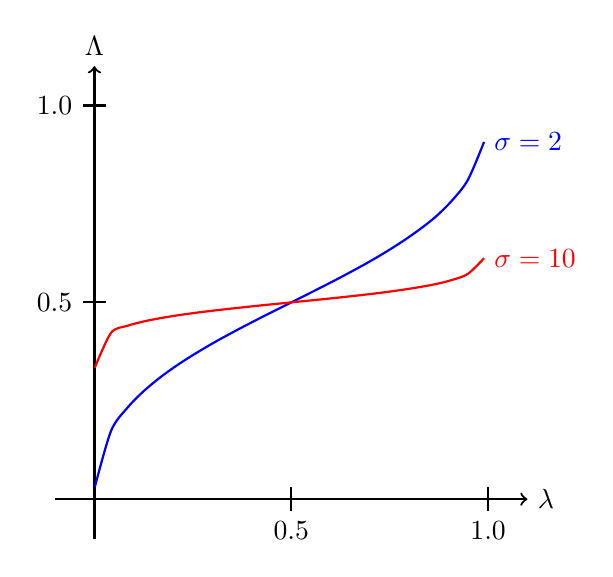
\begin{tikzpicture}[scale=5.0, thick]
      \draw[->] (-0.1,0) -- (1.1,0) node[right] {$\lambda$};
      \draw[->] (0,-0.1) -- (0,1.1) node[above] {$\Lambda$};
      \draw[-]  (0.03,0.5) -- (-0.03,0.5) node[left] {0.5};
      \draw[-]  (0.03,1.0) -- (-0.03,1.0) node[left] {1.0};
      \draw[-]  (1.0,0.03) -- (1.0,-0.03) node[below] {1.0};
      \draw[-]  (0.5,0.03) -- (0.5,-0.03) node[below] {0.5};
      \draw[scale=1.0,domain=0.001:0.99,smooth,variable=\x,blue] plot ({\x},{1 / (1 + ( (1-\x)/\x )^(1/2) )   }) node[right]{$\sigma=2$};
      \draw[scale=1.0,domain=0.001:0.99,smooth,variable=\x,red] plot ({\x},{1 / (1 + ( (1-\x)/\x )^(1/10) )   }) node[right]{$\sigma=10$};
    \end{tikzpicture}
    \end{figure}

 \subsection{Complete markets equilibrium}
 We can work out the prices in this economy using the equivalence of the planner's problem and a competitive equilibrium with complete markets.
 \subsubsection{Terms of trade}
 The terms of trade are
 \begin{eqnarray}
 % \nonumber % Remove numbering (before each equation)
   p &=& \frac{u_y}{u_x} = \frac{1-\omega}{\omega}\left(\frac{x}{y}\right)^\frac{1}{\gamma}=\frac{1-\omega}{\omega}\left(\frac{X}{Y}\right)^\frac{1}{\gamma} \label{eq:tot}.
 \end{eqnarray}
 When the home country has the relatively better endowment, the price of its imports goes up (or the price of its export goes down). This is a supply side story: when $x$ is relatively abundant, we slide down the demand curve. The strength of the effect depends on how substitutable the goods are. When goods are perfect substitutes $\gamma \rightarrow \infty$ relative supplies do not matter and as gamma approaches one, the terms of trade become more volatile. The demand side of the model is wrapped up in the $\omega$ term, which governs how much agents like $y$ relative to $x$.
 \subsubsection{Real exchange rate}
 To find the real exchange rate, first find the price of consumption in each country,
 \begin{eqnarray}
 % \nonumber % Remove numbering (before each equation)
   P&=&\min_{x,y} x+py\\
    \textrm{s.t.} \;\; 1 &=& \left[ \omega x^{\frac{\gamma-1}{\gamma}} + (1-\omega)y^\frac{\gamma-1}{\gamma} \right]^{\frac{\gamma}{\gamma-1}}
 \end{eqnarray}
 the solution to this problem is
 \begin{eqnarray}
 % \nonumber % Remove numbering (before each equation)
   P =\left[\omega^\gamma+(1-\omega)^\gamma p^{1-\gamma}\right]^\frac{1}{1-\gamma}
 \end{eqnarray}
 which is an average of the price of $x$ and $y$. Given the symmetry in utility, $P^*$ has exactly the same form and the real exchange rate is equal to one always. Not very exciting.

\begin{mybox}{Terms of trade when $\omega \neq \omega^*$}
      Let's pretend for a minute that $\omega \neq \omega^*$. This would effect the allocations and the values of $p$, but the form of the price indexes and the real exchange rate would not change. In this case,
      \begin{eqnarray}
      % \nonumber % Remove numbering (before each equation)
        RER = \frac{P^*}{P} = \frac{\left[\omega^{*\gamma}+(1-\omega^*)^\gamma p^{1-\gamma}\right]^\frac{1}{1-\gamma}}{\left[\omega^\gamma+(1-\omega)^\gamma p^{1-\gamma}\right]^\frac{1}{1-\gamma}}
      \end{eqnarray}
      and now the real exchange rate depends on the terms of trade. A common parameterization is to make the countries mirror images of each other, $1-\omega^*=\omega$ so that each country has the same ``home bias.'' In this case, it can be shown [todo: sort this out] that the linear approximation is
      \begin{eqnarray}
      % \nonumber % Remove numbering (before each equation)
        \widehat{rer}(s^t) = (2\omega-1)\widehat{p}(s^t).
      \end{eqnarray}
      If $\omega>0.5$ (home bias)  the real exchange rate and the terms of trade are positively correlated and $\sigma^2(rer) = (2\omega-1)^2\sigma^2(p)$.  The real exchange rate is less volatile than the terms of trade.
 \end{mybox}

\subsubsection{Trade balance}
The planner's allocations imply trade flows. The nominal trade balance is
\begin{eqnarray}
% \nonumber % Remove numbering (before each equation)
  tb(s^t) &=& x^*-p(s^t)y(s^t)\\
  tb(s^t) &=& (1-\Lambda)X(s^t)-\frac{1-\omega}{\omega}\left(\frac{X(s^t)}{Y(s^t)}\right)^{\frac{1}{\gamma}}\Lambda Y(s^t)\\
  \frac{tb(s^t)}{X(s^t)} &=& (1-\Lambda)-\Lambda\frac{1-\omega}{\omega}\left(\frac{Y(s^t)}{X(s^t)}\right)^{\frac{\gamma-1}{\gamma}}\label{eq:ntb}\\
\end{eqnarray}
If $\gamma>1$ (meaning goods are substitutes), the nominal trade balance is positively correlated with $X$ and negatively correlated with $Y$.  If a country gets a positive shock to its endowment, it saves some of it with the other country.

If $\gamma=1$ (Cobb-Douglas) the trade balance is constant, and depends on $\Lambda$ and $\omega$.

\subsubsection{The terms of trade and the trade balance}
This is a classic question in the literature: How are the terms of trade and the trade balance related?  Does a worsening terms of trade imply a worsening of the trade balance? Suppose the home country receives a shock to its endowment (or productivity, or government spending, or\ldots)

The correlation of the nominal trade balance and the terms of trade depends on $\gamma$.
\begin{itemize}
\item If $\gamma>1$, then from \eqref{eq:tot} we see that an increase in $X$ leads to an increase $p$ and, from \eqref{eq:ntb}, an increase in $X$ leads to an increase in $tb/X$. The correlation is positive.

    \item If $\gamma <1$, increasing $X$ still increases $p$, but it decreases $tb/X$, so the correlation is negative.
\end{itemize}
Suppose we consider a real measure of the trade balance. Let $\bar{p}$ be the fixed ``base year'' price.
\begin{eqnarray}
% \nonumber % Remove numbering (before each equation)
  \overline{tb}(s^t) &=& x^*-\bar{p}y(s^t)=(1-\Lambda)X(s^t)-\bar{p}\Lambda Y(s^t)\\
  \frac{\overline{tb}(s^t)}{X(s^t)} &=& (1-\Lambda)-\Lambda\bar{p}\frac{Y(s^t)}{X(s^t)}
\end{eqnarray}

In this case, the real trade balance and the terms of trade are always positively correlated. The relative price is what matters for the nominal trade balance result. When goods are elastic, the price responds less than quantities do and the trade balance rises. When goods are inelastic the price responds more than quantities and the trade balance falls.

\subsection{Financial autarky}

Now we take the opposite extreme case: trade must be balanced in each period. The allocations from the planner's problem are not relevant here. We need to find the appropriate ones. Start with the first order conditions from each household's problem
\begin{eqnarray}
% \nonumber % Remove numbering (before each equation)
  p(s^t) = \frac{u_x}{u_y} =\frac{1-\omega}{\omega}\left( \frac{x(s^t)}{y(s^t)}\right)^\frac{1}{\gamma}=\frac{u_{x}^*}{u_y^*} = \frac{1-\omega}{\omega}\left(\frac{x^*(s^t)}{y^*(s^t)}\right)^\frac{1}{\gamma}.
\end{eqnarray}
Solve for $x$ or $x^*$ and substitute into the budget constraint \eqref{eq:fa-hbc} or \eqref{eq:fa-fbc} and solve.
\begin{eqnarray}
% \nonumber % Remove numbering (before each equation)
  y(s^t) = X(s^t)\frac{1}{p(s^t)+p(s^t)^{\gamma}(\frac{\omega}{1-\omega})^\gamma} \qquad x(s^t) = X(s^t)\frac{p(s^t)^{\gamma}(\frac{\omega}{1-\omega})^\gamma}{p(s^t)+p(s^t)^{\gamma}(\frac{\omega}{1-\omega})^\gamma}\\
  %
   y^*(s^t) = p(s^t)Y(s^t)\frac{1}{p(s^t)+p(s^t)^{\gamma}(\frac{\omega}{1-\omega})^\gamma} \qquad x^*(s^t) = p(s^t)Y(s^t)\frac{p(s^t)^{\gamma}(\frac{\omega}{1-\omega})^\gamma}{p(s^t)+p(s^t)^{\gamma}(\frac{\omega}{1-\omega})^\gamma}
\end{eqnarray}
Substitute the formulas for $y$ and $y^*$ into the market clearing condition for $y$ to find the price,
\begin{eqnarray}
% \nonumber % Remove numbering (before each equation)
  p(s^t)=\left(\frac{X(s^t)}{Y(s^t)}\right)^\frac{1}{\gamma}\frac{1-\omega}{\omega}
\end{eqnarray}
and now back into allocations,
\begin{eqnarray}
% \nonumber % Remove numbering (before each equation)
  y(s^t) = Y(s^t)\frac{1}{1+\left(\frac{X(s^t)}{Y(s^t)}\right)^{\frac{1}{\gamma}-1}\frac{1-\omega}{\omega}} \qquad x(s^t) = X(s^t)\frac{1}{1+\left(\frac{X(s^t)}{Y(s^t)}\right)^{\frac{1}{\gamma}-1}\frac{1-\omega}{\omega}}\\
  %
   y^*(s^t) = Y(s^t)\frac{\left(\frac{X(s^t)}{Y(s^t)}\right)^{\frac{1}{\gamma}-1}\frac{1-\omega}{\omega}}{1+\left(\frac{X(s^t)}{Y(s^t)}\right)^{\frac{1}{\gamma}-1}\frac{1-\omega}{\omega}} \qquad x^*(s^t) = X(s^t)\frac{\left(\frac{X(s^t)}{Y(s^t)}\right)^{\frac{1}{\gamma}-1}\frac{1-\omega}{\omega}}{1+\left(\frac{X(s^t)}{Y(s^t)}\right)^{\frac{1}{\gamma}-1}\frac{1-\omega}{\omega}}
\end{eqnarray}
Notice from the expression for prices that the ratio of foreign to home incomes in history $s^t$ is
\begin{eqnarray}
% \nonumber % Remove numbering (before each equation)
  \frac{p(s^t)Y(s^t)}{X(s^t)}= \left(\frac{X(s^t)}{Y(s^t)}\right)^{\frac{1}{\gamma}-1}\frac{1-\omega}{\omega}
\end{eqnarray}
and allocations can be written as contingent on the relative income in each period,
\begin{alignat}{5}
% \nonumber % Remove numbering (before each equation)
  y(s^t) &= Y(s^t)\Theta(s^t) &\qquad&&x(s^t) =& X(s^t)\Theta(s^t)\\
  %
   y^*(s^t) &= Y(s^t)\left(1-\Theta(s^t)\right)  &\qquad&&x^*(s^t) =& X(s^t)\left(1-\Theta(s^t)\right),
\end{alignat}
where
\begin{align}
\Theta(s^t) = \frac{1}{1+\left(\frac{X(s^t)}{Y(s^t)}\right)^{1/\gamma-1}\frac{1-\omega}{\omega}}.
\end{align}

Recall that in the complete markets (and planner's) solutions, the shares of the endowments that went to the home country and the foreign country were constant ($\Lambda$ was not a function of $s^t$). Again, everything depends on the value of $\gamma$.
\begin{itemize}

  \item If $\gamma<1$ (gross complements), an increase in $Y$ means that $\Theta$ increases. This means that even though the foreign country has a relatively high endowment, its share of the aggregate resources falls. Some people say ``growth is immiserizing.'' This is an income result: the increase in $Y$ leads to a decrease in $p$ that is large enough that $pY$ falls relative to $X$. [The same is true for the home country, too. An increase in $X$ leads to a fall in $\Theta$.]
  \item If $\gamma>1$ (gross substitutes), an increase in $Y$ means that $\Theta$ falls and the foreign country consumes more of the aggregate endowments. In this case the price falls by less than the rise in $Y$ so the relative income of the home country increases. [The same is true for the home country, too. An increase in $X$ leads to a rise in $\Theta$.]
      \item If $\gamma=1$ (Cobb-Douglas aggregator) relative incomes are constant --- the price adjusts just enough to offset changes in the endowment --- so allocations are constant. Wow, that sounds like the planner's allocation! The terms of trade are providing perfect insurance even though countries cannot trade financial instruments.

          In this case, $\Theta(s^t)=\omega$. Using \eqref{eq:Lambda}, we can find a set of planner's weights that deliver the same allocation as the financial autarky equilibrium with $\gamma=1$,
          \begin{equation}
            \omega = \frac{(1-\lambda)^{-1/\sigma}}{(1-\lambda)^{-1/\sigma}+\lambda^{-1/\sigma}}.
          \end{equation}

    This is pretty special case, and it doesn't take much to break the result (e.g., non-traded goods, capital), but it is a nice demonstration of the insurance aspects of the terms of trade. [Show Cole-Obstfeld (1991) set up and results. ]
\end{itemize}

\subsection{Backus Smith (1993)}
Consider a complete markets, exchange economy in which each country in endowed with a tradable good (x; in contrast to our models so far, this is the same good) and each country is endowed with a country-specific non-traded good $(y, y^*)$. The resource constraints are
\begin{align}
  x(s^t)+x^*(s^t)&=X(s^t)+X^*(s^t)\\
  y(s^t) &= Y(s^t)\\
  y^*(s^t)&=Y^*(s^t).
\end{align}
Preferences have a similar form to before, but let's make a few auxiliary definitions. Define final consumption to be
\begin{align}
c(s^t) &= \left( \omega x(s^t)^\frac{\gamma-1}{\gamma} (1-\omega)y(s^t)^\frac{\gamma-1}{\gamma}\right)^\frac{\gamma}{\gamma-1},
\end{align}
with identical preferences for the foreign country. The utility function is CRRA: $c(s^t)^{1-\sigma}(1-\sigma)^{-1}$. The home household maximizes expected utility
\begin{align}
  \sum_{t=0}^{\infty}\sum_{s^t}\beta^t \pi(s^t)(1-\sigma)^{-1}c(s^t)^{1-\sigma},
\end{align}
subject to the period-zero budget constraint,
\begin{align}
  \sum_{t=0}^\infty\sum_{s^t}m(s^t)\left[ x(s^t)+p(s^t)y(s^t) \right]&=\sum_{t=0}^\infty\sum_{s^t}m(s^t)\left[ X(s^t)+p(s^t)Y(s^t) \right].
\end{align}
The foreing country solves a similar problem with the budget constraint
\begin{align}
  \sum_{t=0}^\infty\sum_{s^t}m(s^t)\left[ x^*(s^t)+p^*(s^t)y^*(s^t) \right]&=\sum_{t=0}^\infty\sum_{s^t}m(s^t)\left[ X^*(s^t)+p^*(s^t)Y^*(s^t) \right].
\end{align}
Notice that the prices of non-traded goods are different across countries, but the price of the traded good is not.

\begin{mybox}{A final goods sector}
We are still considering the aggregator a part of preferences, but we could just as well have assumed that there is a perfectly competitive final good industry that purchases traded and non-traded goods and assembles them into the final good.
\begin{align}
  \max_{x,y} P(s^t)c(s^t) - x(s^t) - p(s^t)y(s^t) \\
  \textrm{s.t.}\;\; c(s^t) = \left( \omega x(s^t)^\frac{\gamma-1}{\gamma} (1-\omega)y(s^t)^\frac{\gamma-1}{\gamma}\right)^\frac{\gamma}{\gamma-1}
\end{align}
Impose that profit is zero, and the input demands for $x$ and $y$ will generate $P$. The household (which sells the endowments to the final good firms) now only chooses how much $c$ to purchase at price $P$. The equilibrium of this model and the one in which the aggregator is part of preferences are identical.
\end{mybox}
The first order conditions are
\begin{align}
  \beta^t\pi(s^t)u_x&=\gamma m(s^t)\\
  \beta^t\pi(s^t)u_y&=\gamma m(s^t)p(s^t)\\
  \beta^t\pi(s^t)u_x^*&=\gamma^* m(s^t)\\
  \beta^t\pi(s^t)u_y^*&=\gamma^* m(s^t)p^*(s^t).
\end{align}
Solve the first order conditions for $m(s^t)$ and $m(s^t)p(s^t)$ and substitute them into the consumption price definitions
\begin{align}
  P(s^t) &= \left[\omega^\gamma m(s^t)^{1-\gamma} + (1-\omega)^\gamma \left(m(s^t)p(s^t)\right)^{1-\gamma}   \right]^\frac{1}{1-\gamma}\\
  P(s^t) &= \frac{\beta^t\pi(s^t)}{\gamma}\left[\omega^\gamma u_x^{1-\gamma} + (1-\omega)^\gamma u_y^{1-\gamma}   \right]^\frac{1}{1-\gamma}\\
  P(s^t) &= \frac{\beta^t\pi(s^t)}{\gamma}\left[\omega^\gamma \left[ (\cdot)^{\frac{\gamma(\sigma-1)}{\gamma-1}-1} \omega x(s^t)^\frac{-1}{\gamma} \right]^{1-\gamma} + (1-\omega)^\gamma \left[ (\cdot)^{\frac{\gamma(\sigma-1)}{\gamma-1}-1} (1-\omega) y(s^t)^\frac{-1}{\gamma} \right]^{1-\gamma}   \right]^\frac{1}{1-\gamma}\\
  P(s^t) &= \frac{\beta^t\pi(s^t)}{\gamma}\left[\omega x(s^t)^\frac{\gamma-1}{\gamma}\left[ (\cdot)^{\frac{\gamma(\sigma-1)}{\gamma-1}-1}   \right]^{1-\gamma} + (1-\omega)y(s^t)^\frac{\gamma-1}{\gamma} \left[ (\cdot)^{\frac{\gamma(\sigma-1)}{\gamma-1}-1}   \right]^{1-\gamma}   \right]^\frac{1}{1-\gamma}\\
  P(s^t) &= \frac{\beta^t\pi(s^t)}{\gamma}\left[\omega x(s^t)^\frac{\gamma-1}{\gamma}+ (1-\omega)y(s^t)^\frac{\gamma-1}{\gamma}    \right]^\frac{1}{1-\gamma} (\cdot)^{\frac{\gamma(\sigma-1)}{\gamma-1}-1}\\
  P(s^t) &= \frac{\beta^t\pi(s^t)}{\gamma}\left[\omega x(s^t)^\frac{\gamma-1}{\gamma}+ (1-\omega)y(s^t)^\frac{\gamma-1}{\gamma}    \right]^\frac{\gamma\sigma}{1-\gamma} = \frac{\beta^t\pi(s^t)}{\gamma}c(s^t)^{-\sigma}
\end{align}
The real exchange rate is [do you see why we needed the non-traded goods?]
\begin{align}
  RER(s^t) &= \frac{P^*(s^t)}{P(s^t)}=\frac{\gamma}{\gamma^*}\left(\frac{c^*(s^t)}{c(s^t)} \right)^{-\sigma} \label{eq:bs-risk-sharing}\\
  \log(RER(s^t)) &= \log(\frac{\gamma}{\gamma^*}) + \sigma \log \left(  \frac{c(s^t)}{c^*(s^t)} \right) \qquad \textrm{[flipped the c/c*]}\\
  \Delta \log(RER(s^t)) &=\sigma \Delta \log \left(  \frac{c(s^t)}{c^*(s^t)} \right).
\end{align}
Since this condition holds in each state, it holds for moments, too. (When they exist.) The model ties together the growth rate of the real exchange rate and the growth rate of relative consumption. Moments to consider: [todo: clean up my growth rates notation]
\begin{enumerate}
  \item Means: $\sigma \mu(\Delta rer_t) = \mu(\Delta c_t/c^*_t)$
  \item Standard deviations: $\sigma \std(\Delta rer_t) = \std(\Delta c_t/c^*_t)$
  %\item Cross sectional variation: $\sigma \Delta rer_t^{us,j} = \Delta c_t^{us}/c^j_t$
\end{enumerate}
The model predicts that as consumptions becomes more expensive, the country should consume less. If $p$ increases, then $p^*/p$ decreases and
These relationships depend on $\sigma$, but the monotonicity of the two growth rates can be tested with cross-section correlations, such as
\begin{align}
  \rho(\sigma \mu(\Delta rer_t^{us,j}), \mu(\Delta c_t^{us}/c^j_t))&=\frac{\cov(\sigma \mu(\Delta rer_t^{us,j}), \mu(\Delta c_t^{us}/c^j_t))}{\std(\sigma \mu(\Delta rer_t^{us,j}))\std(\mu(\Delta c_t^{us}/c^j_t))}\\
  \rho(\sigma \mu(\Delta rer_t^{us,j}), \mu(\Delta c_t^{us}/c^j_t))&=\frac{\sigma \cov(\mu(\Delta rer_t^{us,j}), \mu(\Delta c_t^{us}/c^j_t))}{\sigma\std( \mu(\Delta rer_t^{us,j}))\std(\mu(\Delta c_t^{us}/c^j_t))}\\
  \rho(\sigma \mu(\Delta rer_t^{us,j}), \mu(\Delta c_t^{us}/c^j_t))&=\rho(\mu(\Delta rer_t^{us,j}), \mu(\Delta c_t^{us}/c^j_t))
\end{align}
which does not depend on $\sigma$.

[Show figures from BS]

\begin{itemize}
  \item rer is more volatile than consumption
  \item autocorrelation of consumption negative, of rer positive
  \item means might be about right?
\end{itemize}
The Backus-Smith Puzzle is that $\rho(\Delta rer_t, \Delta c_t/c^*_t)$ is negative in the data and positive in the model.
Corsetti Dedola Leduc extend to larger, more recent sample. Confirm puzzle.

Fixing the puzzle involves breaking fundamental risk-sharing relationship in \eqref{eq:bs-risk-sharing}. One way to do so is to make preferences assymetric: different sigma, betas; this is Coleman's thesis. Another way is to introduce wealth effects through incomplete markets. Epstein Zin preferences make Pareto weights move. [Do Backus and the kids paper?]

\section{Two country models with production}
The canonical two country international business sector.
\subsection{The model}
The economy consists of two equally-sized countries, home and foreign. Each county features a representative household, and, in some cases, a government. The home country produces the $a$ good and the foreign country produces the $b$ good. Goods $a$ and $b$ are tradable. They are combined to form a nontradable final good in each country.

We focus on the model with complete markets, so that we can solve the planner's problem. We begin by laying out the resource constraints.

\subsubsection*{Intermediate goods}
Intermediate good production in each country is Cobb-Douglas. Each country uses $a$ and $b$ in production of the final good. The resource constraints for the two goods are
\begin{align}
  a(s^t) + a^*(s^t) &= \exp(z(s^t))k(s^t)^\alpha \ell(s^t)^{1-\alpha}\label{eq:irbc-intermediate-1}\\
  b(s^t) + b^*(s^t) &= \exp(z^*(s^t))k^*(s^t)^\alpha \ell^*(s^t)^{1-\alpha}
\end{align}
where $z$ is stochastic productivity --- the source of fluctuations in the economy. [These shocks affect real variables, and hence the whole ``real'' business cycle language.] $k$ is capital and $\ell$ is labor.

We have no trade costs in this model, but if we included them (and they were iceberg costs, not tariffs!) they would show up here.

\subsubsection*{Productivity}
The $z$ process is AR(1)
\begin{equation}\label{eq:irbc-z-ar1}
 \left [ \begin{tabular}{l}
    $z(s^t)$\\
    $z^*(s^t)$
    \end{tabular}
    \right ] =
    A\left [ \begin{tabular}{l}
    $z(s^{t-1})$\\
    $z^*(s^{t-1})$
    \end{tabular}
    \right ]
    +
    \left [ \begin{tabular}{l}
    $\epsilon(s^{t})$\\
    $\epsilon^*(s^{t})$
    \end{tabular}
    \right ]
\end{equation}

\begin{equation}
 \left [ \begin{tabular}{l}
    $\epsilon(s^t)$\\
    $\epsilon^*(s^t)$
    \end{tabular}
    \right ] \sim
    N \left(
    \left[\begin{tabular}{l}
    $0$\\
    $0$
    \end{tabular}
    \right]
    ,\sigma^2_{\epsilon_z}
    \left[
    \begin{tabular}{ll}
    $1$&$\rho_{\epsilon_z}$\\
    $\rho_{\epsilon_z}$&$1$
    \end{tabular}
    \right]
    \right)
\end{equation}

The off diagonal elements of $A$ generate spillovers. If $a_{11}=a_{22}>0$, an increase in productivity in one country will lead to a increase in productivity in the other country (with a lag). This is one way to generate correlated productivity.

The shock process allows for the other way to generate correlated productivity. When $\rho_{\epsilon_z} \neq 0$ the innovations to the productivity are correlated. These are ``global shocks.'' Both spillovers and global shocks generate productivity --- and thus output -- cross country correlation, but they are fundamentally different mechanisms.


\subsubsection*{Final goods}
Final good production combines $a$ and $b$ using a CES aggregator. The home and foreign final good resource constraints are
\begin{align}\label{eq:irbc-final-rc}
  c(s^t)+x(s^t) &= \left(\omega^\frac{1}{\gamma}a(s^t)^\frac{\gamma-1}{\gamma}+ (1-\omega)^\frac{1}{\gamma}b(s^t)^\frac{\gamma-1}{\gamma}\right)^\frac{\gamma}{\gamma-1}\\
  c^*(s^t)+x^*(s^t) &= \left(\omega^\frac{1}{\gamma}b^*(s^t)^\frac{\gamma-1}{\gamma}+ (1-\omega)^\frac{1}{\gamma}a^*(s^t)^\frac{\gamma-1}{\gamma} \right)^\frac{\gamma}{\gamma-1}
\end{align}
Note the symmetry in the CES aggregators. The $\omega$ and $\gamma$ are common --- the only difference is that the positions of $a$ and $b$ are swapped. When $\omega>0.5$, each country uses more of its locally produced good. This is a feature of the data known as \textit{home bias}.

Capital accumulation follows the usual law of motion. Notice that there are not Lucas and Prescott style adjustment frictions.
\begin{align}
  k(s^{t+1}) &= k(s^t)\left(1-\delta\right)+x(s^t) \label{eq:irbc-lomk-1}\\
  k^*(s^{t+1}) &= k^*(s^t)\left(1-\delta\right)+x^*(s^t)\label{eq:irbc-lomk-2}
\end{align}

\subsection{The planner's problem}
The planner weights the home country with $\lambda$ and the foreign country with $\lambda^*$. The planners problem is choose sequences of $c,c^*,\ell, \ell^*, k, k^*, x, x^*$ to maximize
\begin{equation}\label{eq:irbc-planner-problem}
   \sum_{t=0}^\infty \sum_{s^t} \beta^t \pi(s^t)\left[\lambda u\left(c\left(s^t\right),\ell\left(s^t\right) \right) + \lambda^* u\left(c^*\left(s^t\right),\ell^*\left(s^t\right) \right) \right]
\end{equation}
subject to the resource constraints (\ref{eq:irbc-intermediate-1}--\ref{eq:irbc-lomk-2}).

Let $\nu$ be the multiplier on the final good constraint, $\mu$ the multiplier on the intermediate good constraint, and let $\eta$ be the multiplier on the law of motion for capital. The intra-temporal first order conditions are
\begin{align}
  [c:]&&\lambda \beta^t \pi(s^t) u_c(s^t) &= \nu(s^t) & \lambda^* \beta^t \pi(s^t) u_c^*(s^t) &= \nu^*(s^t)\\
  [\ell:]&&\lambda \beta^t \pi(s^t) u_\ell(s^t) &= \mu(s^t)F_\ell(s^t) & \lambda^* \beta^t \pi(s^t) u_\ell^*(s^t) &= \mu^*(s^t)F^*_\ell(s^t)\\
  [a:]&&\mu(s^t) &= \nu(s^t)D_{a}(s^t) & \mu(s^t) &= \nu^*(s^t)D_{a^*}(s^t)\\
  [b:]&&\mu^*(s^t) &= \nu(s^t)D_{b}(s^t) & \mu^*(s^t) &= \nu^*(s^t)D_{b^*}(s^t)\\
  [x:]&&\eta(s^t) &= \mu(s^t) & \eta^*(s^t) &= \mu^*(s^t)
\end{align}
and the inter-temporal first order conditions are
\begin{align}
  [k:]&&\eta(s^t) &= \sum_{s^{t+1}}\left\{ (1-\delta)\eta(s^{t+1})+\mu(s^{t+1})F_k(s^{t+1}) \right\}\\
  [k^*:]&&\eta^*(s^t) &= \sum_{s^{t+1}}\left\{ (1-\delta)\eta^*(s^{t+1})+\mu^*(s^{t+1})F_k^*(s^{t+1}) \right\}
\end{align}
Combining equations, we arrive at the familiar relationships. The first is the intra-temporal tradeoff between consumption and leisure,
\begin{align}
  \frac{u_c(s^t)}{u_\ell(s^t)} &= \frac{1}{D_a(s^t)F_\ell(s^t)}\\
  \frac{u_c^*(s^t)}{u_\ell^*(s^t)} &= \frac{1}{D_b(s^t)F_\ell^*(s^t)}.
\end{align}
This equates the ratio of the marginal utility from consumption and leisure with the relative price. The ``1'' in the numerator on the right hand side is the price of consumption (the numeraire) and the denominator is the wage. The wage is the marginal product of labor ($F_\ell$) evaluated at its marginal contribution to consumption ($D_a$).

The Euler equations give us the usual tradeoff between consuming today or investing in a unit of capital that is productive in the next period,
\begin{align}
  u_c(s^t) & =\beta \EX_t\left\{ \left(1-\delta+F_k(s^{t+1})D_a(s^{t+1}) \right)u_c(s^{t+1})   \right\}\\
  u_c^*(s^t) & =\beta \EX_t\left\{ \left(1-\delta+F_k^*(s^{t+1})D_b^*(s^{t+1}) \right)u_c^*(s^{t+1})   \right\}.
\end{align}
The marginal cost of the investment is the foregone consumption at $t$, which is the left hand side of the Euler equation. The expected benefit is the right hand side of the equation. It is the net (of depreciation) return on capital (evaluated at its marginal contribution to consumption) times the marginal utility of future consumption.

Lastly, we have the risk sharing condition,
\begin{align}
  \lambda u_c(s^t)D_a(s^t) &= \lambda^*u_c^*(s^t)D_a^*(s^t)\\
  \lambda u_c(s^t)D_b(s^t) &= \lambda^*u_c^*(s^t)D_b^*(s^t).
\end{align}
This says that, state-by-state, the planner equates (up to the weights) the marginal utility from $a$ and $b$. $a$ and $b$ are the two goods that can be traded, so the planner allocates the goods across the countries until the marginal consumption value is equalized. The $u$ and $D$ functions are functions of both $a$ and $b$ and also $\ell$ and $c$, so these are complex conditions.

\subsubsection*{Prices and trade flows}
After solving the planner's problem, we can recover prices and trade flows in the usual way. The home country terms of trade are
\begin{equation}
  p(s^t)=\frac{q_b(s^t)}{q_a(s^t)}=\frac{D_b(s^t)}{D_a(s^t)}.
\end{equation}
The real exchange rate is the usual function of the terms of trade,
\begin{equation}
  rer(s^t) = \frac{P^*(s^t)}{P(s^t)}=\frac{\left( \omega p(s^t)^{1-\gamma}+(1-\omega) \right)^\frac{1}{1-\gamma}}{\left( \omega +(1-\omega)p(s^t)^{1-\gamma} \right)^\frac{1}{1-\gamma}}.
\end{equation}
Notice that the aggregate price indexes are weighted averages of the terms of trade. This suggests that the real exchange rate will be less volatile than the terms of trade. This is going to be problematic when we compare the model to the data.

The net export to GDP ratio is
\begin{equation}
  nxy(s^t)=\frac{a^*(s^t)-p(s^t)b(s^t)}{a(s^t)+a^*(s^t)}.
\end{equation}
\subsection{Calibration}
The model period is one quarter. The steady state Euler equation is
\begin{equation}\label{}
  \frac{1}{\beta} = 1-\delta+F_k
\end{equation}
so that the net interest rate is $\beta^{-1}$. Set $\beta=0.99$ to make the quarterly interest rate 1 percent. A constant returns to scale, perfectly competitive intermediate good firm would imply that
\begin{equation}
  \frac{w(s^t)\ell(s^t)}{a(s^t)+a^*(s^t)}=\alpha,
\end{equation}
so $\alpha=0.36$, which is the U.S. average labor share. [There has been a lot of discussion about the stability of the labor share recently.] In the NIPA accounts, capital consumption allowance is the counterpart to $\delta k(s^t)$. Set $\delta=0.025$ to match the quarterly data.

The utility function is [todo: $\mu$ is a multiplier in the planner's problem]
\begin{equation}\label{eq:standard-prefs}
  u(c,\ell) = (1-\sigma)^{-1}\left[ c^\mu (1-\ell)^{1-\mu} \right]^{1-\sigma}.
\end{equation}
Take $\sigma=2$ as given. Set $\mu=0.34$ so that steady-state $\ell$ is about 1/3 of the time endowment. [Todo: add the algebra.]

The most important parameter turns out to be $\gamma$, the elasticity of substitution between home and foreign goods. It is a parameter that doesn't really have a single value. Estimates range from 0.25 to 20, depending on the variation used to identify the parameter and whether the estimate is capturing a short or long term adjustment. As a baseline, set $\gamma=1.5$ (which a ``trade'' economists would think is nuts) and set units in the steady state so that $p=1$. The first order conditions imply, in the steady state, that
\begin{equation}\label{}
  \left(\frac{\omega}{1-\omega}\right)^\gamma=\frac{1-\frac{b}{a+a^*}}{\frac{b}{a+a^*}}
\end{equation}
where $b/(a+a^*)$ is the import to GDP ratio. If the import share is about 0.15 so $\omega=0.76$.

\subsubsection*{Productivity}
The productivity shocks are estimated from the Solow residuals. Take home to the the United States and foreign to be an aggregate of the Europe or maybe the OECD. We are looking for roughly symmetrical countries. Impose symmetry on the system and estimate.

BKK find $a_{11}=a_{22}=0.906$ and $a_{12}=a_{21}=0.088$. As usual, productivity is persistent. The off diagonal elements are positive and small --- there are small, positive spillovers. They are usually barely statistically significant, or not significant at all.

The innovation to productivity has $\sigma_{\epsilon_z}=0.085$ and $\rho_{\epsilon_z}=0.258$. There is some tendency to global shocks.

\subsection{Results}
Show impulse response functions.

An increase in home country productivity:
\begin{itemize}
  \item Hours worked has two effects: income and substitution effect. At home, productivity is relatively high, so you want to work more. Income goes up, so you want to work less. Substitution effect wins out and home works more. Abroad, productivity is relatively low, so both effects more in same direction. Initially work less. As productivity spills over, start working more.
  \item Investment in the home country immediately increases. The future productivity of capital is relatively high, so you want more future capital stock. Abroad, investment initially falls. Capital is relatively more productive abroad, so shift resources there.
  \item Output increases in the home country (labor supply increases and the productivity is high). It falls in the foreign country initially (labor supply falls) and rises as labor supply and productivity increase.
  \item Consumption increases in both countries, but not by the same amount. Preferences are not additively separable in leisure and consumption, so we get positive correlation across countries, but not perfect correlation.
\end{itemize}

\textbf{The trade elasticity}\\
BKK stress the importance of the elasticity of substitution between home and foreign goods, $\gamma$ for the behavior of relative prices and the trade balance.

\begin{itemize}
\item When $\gamma$ is small, $\corr(p_t,nxy_t)<0$. The goods are poor substitutes. An increase in home productivity increases the supply of $a$ which drives up the relative  price of $b$, $p$. Since goods are poor substitutes, however, the agents do not want to deviate much from the steady state $a$-to-$b$ ratio (see Figure~\ref{fig:optimal-mix}). The home country demands imports and pays a lot for them. This means that an increase in $p$ leads to a decrease in $nxy$.
\item When $\gamma$ is large, $\corr(p_t,nxy_t)>0$. The goods are close substitutes. An increase in the supply of $a$  leads to an increase in$p$, but not by much. The home agent substitutes away from $b$ while still sending some of the cheaper $a$ abroad (the foreign country would like cheap $a$, too). If $gamma$ is large enough, the quantity response outweighs the price response and net exports can be come more positive.
\item Note the implications for volatility. When $gamma$ is small, prices are volatile and quantities are not. When $\gamma$ is large, prices are not very volatile and quantities are volatile (real quantities, not $nxy$).
\end{itemize}
 \begin{figure}[H]
 \centering
 \caption{Optimal mix of imports and domestic goods, $\omega=0.5$} \label{fig:optimal-mix}
 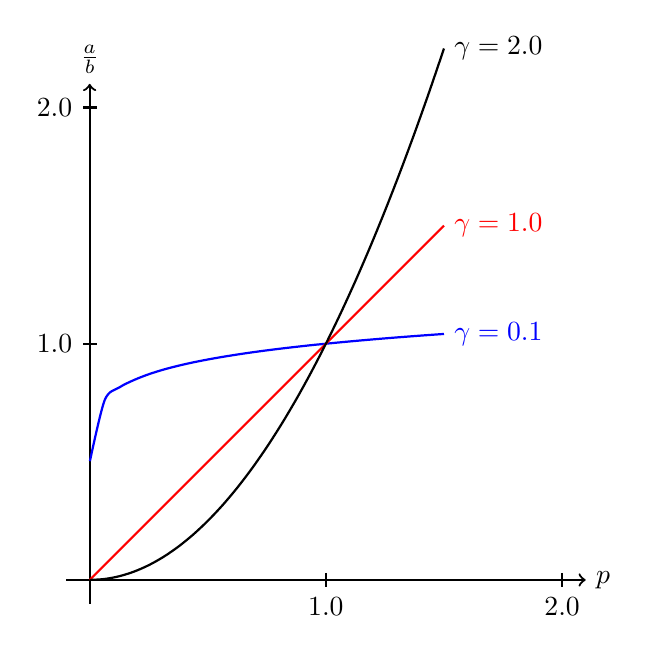
\begin{tikzpicture}[scale=3.0, thick]
      \draw[->] (-0.1,0) -- (2.1,0) node[right] {$p$};
      \draw[->] (0,-0.1) -- (0,2.1) node[above] {$\frac{a}{b}$};
      %\draw[-]  (0.03,0.5) -- (-0.03,0.5) node[left] {0.5};
      \draw[-]  (0.03,1.0) -- (-0.03,1.0) node[left] {1.0};
      \draw[-]  (0.03,2.0) -- (-0.03,2.0) node[left] {2.0};
      \draw[-]  (1.0,0.03) -- (1.0,-0.03) node[below] {1.0};
      \draw[-]  (2.0,0.03) -- (2.0,-0.03) node[below] {2.0};
      \draw[scale=1.0,domain=0.001:1.5,smooth,variable=\x,blue] plot ({\x},{\x^(0.1)}) node[right]{$\gamma=0.1$};
      \draw[scale=1.0,domain=0.001:1.5,smooth,variable=\x,red] plot ({\x},{\x^(1)}) node[right]{$\gamma=1.0$};
      \draw[scale=1.0,domain=0.001:1.5,smooth,variable=\x,black] plot ({\x},{\x^(2)}) node[right]{$\gamma=2.0$};
    \end{tikzpicture}
    \end{figure}

\begin{figure}
  \centering
  \caption{From Backus, Kehoe, and Kydland (1994)}\label{fig:bkk-elas}
  \includegraphics[width=\textwidth]{figures/bkk_elasticity.pdf}
\end{figure}

\FloatBarrier
\section{Heathcote and Perri (2002)}
Notes on  your slides printouts. Type them up.

\section{Raffo 2008}
Data facts
\begin{enumerate}
\item \textbf{Nominal net exports are counter-cyclical (table 1).} This implies that countries borrow during expansions, rather than save to smooth consumption.

\item \textbf{Real net exports drive nominal net exports.} Table 2 says that this is driven by counter-cyclical real net exports and that the terms of trade are mostly acyclical.

\item \textbf{Domestic absorption is move volatile than output.} Domestic absorption is output minus net exports,
\begin{align}
  d_t &= y_t-nx_t\\
  \var(d_t) &= \var(y_t) + \var(nx_t) - 2\cov(y_t,nx_t)
\end{align}
since $\cov(y_t,nx_t)<0$, then it must be that
\begin{align}
  \var(d_t) > \var(y_t).
\end{align}
 \end{enumerate}

 \subsection{What's wrong with BKK?}
 Fire up the BKK model, right from their paper, except add investment frictions. [This is a bit weird. BKK do a pretty good job of hitting investment volatility in their paper, but they have a larger investment volatility in the data. Look into this\ldots]

 Figure 1 shows that $nxy$ is counter-cyclical, but only because the terms of trade move a lot. $rnxy$ is slightly procyclical. This also implies that the volatility of output is greater than domestic absorption. [Duh, it's an identity.]

 What's going wrong? Consumption, which is 80 percent of expenditure, is too smooth (lines 1 and 2 in table 4). Real net exports are procyclical for consumption smoothing purposes. This is against the BKK intuition.

 \subsection{Fixing BKK}
 Let's jack up consumption volatility. Introduce GHH preferences, $c-\psi\ell^\nu$. These preferences kill off the wealth effect on labor. From the first order condition
 \begin{equation}\label{}
 \ell(s^t)=\frac{1}{\psi\nu}w(s^t)^\frac{1}{\nu-1}.
 \end{equation}
 The Frisch labor supply elasticity  is $\epsilon=1/(\nu-1)$.\footnote{The Frisch elasticity is the elasticity of labor supply with respect to the wage holding the marginal utility of wealth constant, $\epsilon = u_\ell/(\ell u_{\ell\ell}-\ell\frac{u_{\ell c}^2}{u_{cc}})$. } In preferences like those in \eqref{eq:standard-prefs}, the Frisch elasticity depends on how much the agent is working,
 \begin{equation}\label{}
   \epsilon = \frac{(1-\ell(s^t))[1-\mu(1-\gamma)]}{\gamma\ell(s^t)}.
 \end{equation}
 When the wage increases, people work more. People don't like working, though so they consume more to compensate. This increases the volatility of consumption relative to ``standard'' preferences. [Include some note about home production.]

 Recalibrate the model so that the Frisch labor supply elasticity is the same as in BKK and so that investment volatility is the same. It is important to get investment volatility right, since the focus in on consumption volatility.

 Along other dimensions (Table 7), quasi-linear preferences bring the model closer to the data on the cross-country correlation of labor inputs. It doesn't help with the cross-country correlations of investment, output, or consumption. The ``quantity anomaly'' remains.
\end{document} 